\newpage
\section{Zusammenhang Graphentheorie und GraphQL}
\label{graphtheorieQL}

Da ein grundlegendes Wissen über Graphentheorie und GraphQL geschaffen wurde, muss noch gezeigt werden, dass Graphentheorie auch anwendbar ist auf GraphQL.
Die Verknüpfung wird später genutzt, um Algorithmen, die für Graphen gedacht sind, für GraphQL zu nutzen.

\subsection{Schema als Graph}

Das GraphQL-Schema ist, wie im Kapitel~\ref{schematypes} gezeigt, eine Komposition von Typen.
Ein Typ definiert Felder in sich.
Jedes Feld eines Typens zeigt seinerseits wieder auf ein anderes Feld~\cite[vgl. Modelling with GraphQL]{graphqlgraphtheory}.
Somit wird jedes Feld eines Typens zu einer ausgehenden Kante.
Es sei ein einfacher Typ $Buch$ mit zwei Feldern vom Typ $SCALAR$ in Abbildung~\ref{kek} definiert.
Der zugehörige Graph ist dargestellt in Abbildung~\ref{kekl}.

\begin{figure}[ht]
    \centering
    \begin{minipage}[h]{0.45\textwidth}
        \begin{verbatim}
        type Buch {
            id: Int
            title: String
        }
        \end{verbatim}
        \caption{Buch-Typ}
        \label{kek}
    \end{minipage}
    \hfill
    \begin{minipage}[h]{0.45\textwidth}
        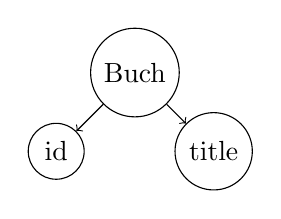
\begin{tikzpicture}
            \node[circle, draw] (n1) at (1,1) {Buch};
            \node[circle, draw] (n2) at (0,0) {id};
            \node[circle, draw] (n3) at (2,0) {title};
            \draw[->] (n1) -- (n2);
            \draw[->] (n1) -- (n3);
        \end{tikzpicture}
        \caption{Graph des Typ-Buch}
        \label{kekl}
    \end{minipage}
\end{figure}

Der Typ $Buch$ besitzt zwei ausgehende Kanten, zu den jeweils beiden definierten Feldern $id$ und $title$.
In Kapitel~\ref{schematypes} wurde festgestellt, dass Skalare Typen keine eigenen Beziehungen haben.
Daher können die Felder $id$ und $title$ selbst keine ausgehenden Kanten haben.
Das generelle Prinzip der Graphbildung ist:

\begin{enumerate}
    \item Erstelle Knoten aus jedem Typen und den definierten Feldern des Knotens.
    \item Ziehe für jeden Typ seine Kanten, indem alle Felder des Typens zum entsprechenden Knoten verbunden werden.
\end{enumerate}
Nach diesem Prinzip kann aus einem beliebig großen Schema ein gerichteter Graph gebildet werden.
\newpage


\subsection{Abfragen im Graphen}
\label{abfrgraph}

Im Folgenden soll geklärt werden, wie GraphQL Anfragen intern behandelt und dies abbildbar in einem Graphen ist.
Hierfür wird in Abbildung~\ref{schemdef} ein Schema definiert.

\begin{figure}[htb]
    \centering
    \begin{minipage}[h!tb]{0.4\textwidth}
        \begin{lstlisting}[language=GraphQL]
type Query {
    buch: Buch
    autor: Autor
}
type Buch {
    id: Int
    title: String
    autor: Autor
    verleger: Verlag
}
        \end{lstlisting}
    \end{minipage}
    \hfill
    \begin{minipage}[h!tb]{0.4\textwidth}
        \begin{lstlisting}[language=GraphQL]
type Author {
    id: Int
    name: String
    schrieb: [Buch!]
}
type Verlag {
    name: String
}
        \end{lstlisting}
    \end{minipage}
    \caption{Schemadefinition}
    \label{schemdef}
\end{figure}

Das in Abbildung~\ref{schemdef} definierte Schema wird durch den Graphen in Abbildung~\ref{schemg} visualisiert.

\begin{figure}[htb]
    \centering
    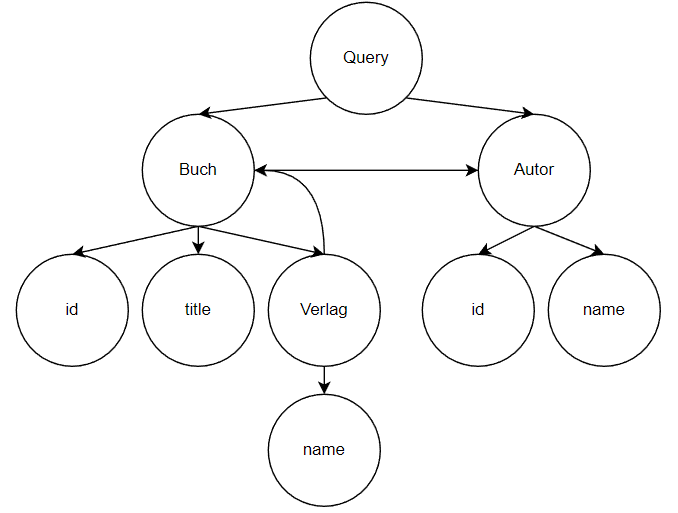
\includegraphics[width=\textwidth,height=0.4\textheight,keepaspectratio]{img/graph}
    \caption{Graph für Schemadefinition aus Abbildung~\ref{schemdef}}
    \label{schemg}
\end{figure}

Valide Anfragen an eine GraphQL-API sind alle Pfade, die mit Startknoten $Query$ beginnen und mindestens einen Knoten beinhalten,
der keine ausgehenden Kanten hat (also ein Scalar-Type)~\cite[vgl. Modelling with GraphQL]{graphqlgraphtheory}.
Auf jeder Ebene des Graphens werden Resolver ausgeführt, welche für die Datenbereitstellung verantwortlich sind.
Es ist wichtig zu betonen, dass der aufgespannte Graph ein gerichteter Graph ist.
Hierdurch wird ermöglicht, dass die $SCALAR$ Felder stets Endknoten sind da sie selbst keine ausgehenden Kanten besitzen dürfen.
Soll von einem GraphQL-Server mit dem zuvor definierten Schema ein Buch mit id, Titel und Verlag mit Verlagsnamen abgefragt werden,
so kann diese Query genutzt werden: \verb+{ buch { id title verleger { name }}}+.

\begin{figure}[htb]
    \centering
    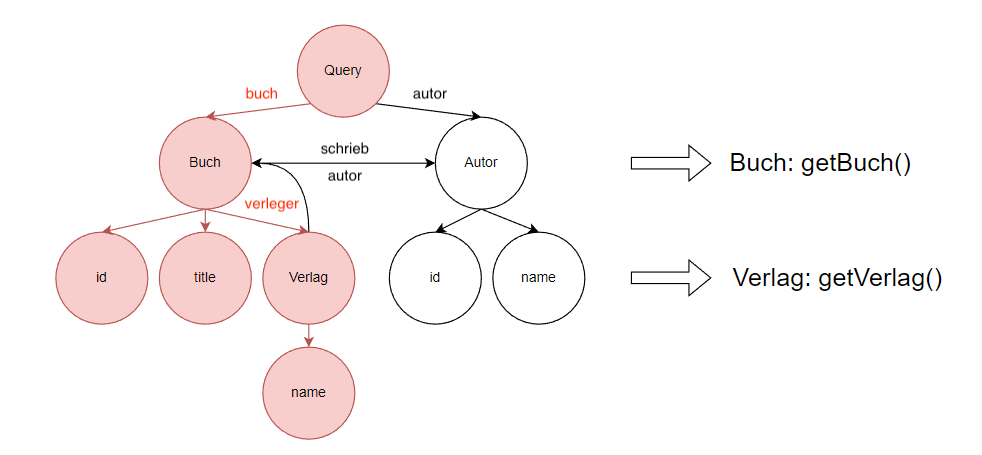
\includegraphics[width=\textwidth,height=0.4\textheight,keepaspectratio]{img/graphresolver}
    \caption{Graph für Abfrage nach~\cite{graphqlgraphtheory}}
    \label{abfrage}
\end{figure}

Mit Ausführung dieser Query wird zuerst der Resolver $getBuch()$ ausgeführt.
Liefert dieser ein valides Ergebnis zurück, also gibt es ein solches Buch, dann wird der nächste Resolver $getVerlag()$ ausgeführt~\cite[vgl. Resolver]{graphqlgraphtheory}.
Dadurch, dass die Typen $Buch$ und $Autor$ aufeinander verweisen, ist der Graph des Schemas zyklisch und die Pfadmenge,
das heißt die erlaubten Abfragen, die gestellt werden können, unendlich.
